\documentclass[prl,twocolumn]{revtex4-1}

\usepackage{graphicx}
\usepackage{color}
\usepackage{comment}
\usepackage{latexsym,amsmath}
\usepackage{verbatim}
\usepackage{listings}
\usepackage{xcolor}

\definecolor{codegreen}{rgb}{0,0.6,0}
\definecolor{codegray}{rgb}{0.5,0.5,0.5}
\definecolor{codepurple}{rgb}{0.58,0,0.82}
\definecolor{backcolour}{rgb}{0.95,0.95,0.92}
\definecolor{commentsColor}{rgb}{0.497495, 0.497587, 0.497464}
\definecolor{keywordsColor}{rgb}{0.000000, 0.000000, 0.635294}
\definecolor{stringColor}{rgb}{0.558215, 0.000000, 0.135316}

\definecolor{deepblue}{rgb}{0,0,0.5}
\definecolor{deepred}{rgb}{0.6,0,0}
\definecolor{deepgreen}{rgb}{0,0.5,0}
\definecolor{linkcolor}{rgb}{0,0,0.65} %hyperlink

\colorlet{keyword}{blue!100!black!80}
\colorlet{comment}{green!90!black!90}
%\usepackage{listings}
\usepackage[pdftex,colorlinks=true, pdfstartview=FitV, linkcolor= linkcolor, citecolor= linkcolor, urlcolor= linkcolor, hyperindex=true,hyperfigures=true]{hyperref} %hyperlink%

\lstdefinestyle{python}{
    backgroundcolor=\color{backcolour},   
    commentstyle=\color{comment},
    keywordstyle=\color{keyword},
    numberstyle=\tiny\color{codegray},
    stringstyle=\color{codepurple},
    basicstyle=\ttfamily\scriptsize,
    breakatwhitespace=false,         
    breaklines=true,                 
    captionpos=b,                    
    keepspaces=true,                 
    numbers=left,                    
    numbersep=5pt,                  
    showspaces=false,                
    showstringspaces=false,
    showtabs=false,                  
    tabsize=2,
    numberstyle=\tiny
}


\begin{document}

\title{2216 -- A deep dive into Neural Networks for 2-dimensional Binary Classification}
% \title{2216 -- The hunt for the golden Neural Network for Classifying a Triangle}

\author{Ema Baci}
\author{Christoffer Askvik Faugstad}
\author{Veslemøy Therese Svendby Osmundsen}

\date{\today}

\begin{abstract}
An investigation was done to determine how different hyper parameters in a deep neural network impacts its performance. The architecture of the network, training parameters and initialization of the layers in the model was tuned by using grid search, yielding the best possible model for the task. It was found that a smaller sample size for training is sufficient to yield a good accuracy as long as the number of epochs is increased, and that augmentation of data serves well as an artificial generator of more samples. For the simple task of binary classification of points, several combinations of parameters yielded good results which indicated that a very complex network is not necessary for such a simple task.

\end{abstract}

\maketitle

\section{Introduction}
Neural Networks (NN) are the new standard for data classification and regression, but the more modern approaches include many advanced features and their effects may be hard to grasp. Even the naive fully connected forward feed NN have many possible design choices and parameters that affects its performance. To understand what their influences are, it is best to study a known, simple problem. Therefore, binary two dimensional samples taken from a known distribution, binary classified by a known non-linear function, was studied. This allows for simple visualization and evaluation of the NN performance.

% In this task a sequential deep neural network was built to perform binary classification of two dimensional points. The aim was to predict whether a given point in a grid of size $\left[-50,50\right]$ was classified within the boundaries of a chosen shape or pattern. In our experiments a triangle was used as the geometrical shape, and hence the final network model was tuned for that purpose. The network parameters chosen may also work well for training of other simple shapes, but for more complex patterns, a more complex model is needed. Nevertheless, the triangle works well to show the impact of the different parameters on the network.

%%%%%%%%%%%%%%%%%%%
%\begin{figure*}[!tb]
%  \centering
%%  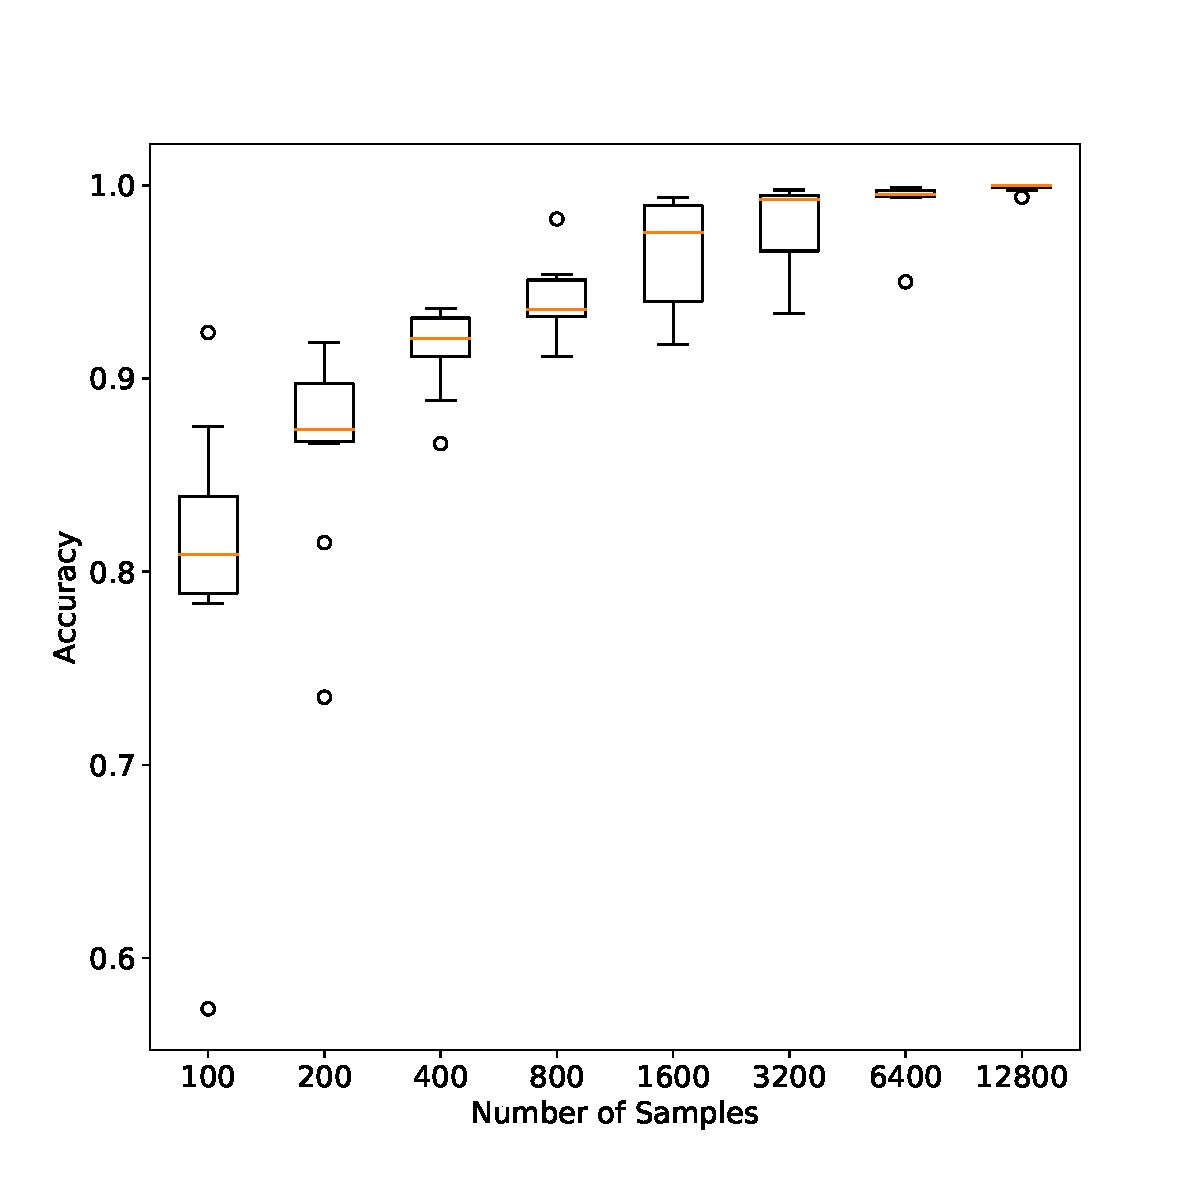
\includegraphics[width=0.3\textwidth]{task_1/num_train_box.pdf}
%  \caption{Description of the panels: (a)..... (b)... etc. This %caption should give enough info on the content of figures to %make them mostly readable without consulting the main text. %However, repetitions with the main text should e avoided if %possible. {\color{red} If this format is difficult to frame in %the page you want, just break it into multiple single %figures.}}
%  \label{fig:x}
%\end{figure*}
%%%%%%%%%%%%%%%%%%%

\section{Methods}
In order to optimize the network, many parameters needed to be taken into consideration. First of all, the number of samples required to train the network sufficiently was considered to determine the training set size that would optimize both the accuracy and the computational time. Next, the effect of adding augmented samples to the training set as a substitute for more generated data was investigated, as well as different ways of scaling the data. The performance of the NN was then further improved through a Grid Search Validation process, which led to the best parameters and the optimization of the initial weights.
%\subsection{Problem} % Not to be kept
%A binary classification problem in two dimensions is considered where the samples are labeled by a non-linear function. The samples have each component drawn uniformly and uncorrelated from the range $[-50,50]$. The main non-linear function used is the triangle, described by the function 
%\begin{equation}
%f(x_1,x_2) = \begin{cases} 1,\
%x_1\in [-20,80] \wedge x_2 \in [-40,80-x_1]\\
%0, \ \textrm{else}.
%\end{cases}
%\end{equation}
%Other functions used for labeling are shown in figure
% \ref{fig:domains}. % Not sure if this should be present.
%They are used to see how the found network performs on a more complex function. 
%\\
% \subsection{The Neural Network architecture}
%\vspace{0.5 cm}
\vskip 4pt
The network model was created by using \texttt{Keras.Sequential()}, which yields a fully connected NN. The hidden layers were of the type \texttt{Dense}, each subject to a set dropout rate. For the final layer the activation function sigmoid was used. The remaining parameters in need of being determined for the NN are given in Table \ref{tab:parameters}.

\begin{table}[!ht]
\begin{center}
\begin{tabular}{lllll}
\hline
Parameters\\
\hline
Number of hidden layers\\
Initialization of weights\\
Activation function\\
Dropout rate\\
Learning rate \\
Batch size \\
Number of epochs \\
\hline
\end{tabular}
\end{center}
\caption{The parameters investigated to optimize the performance of the neural network.}
\label{tab:parameters}
\end{table}

%The initial parameters chosen are reported below:

% \begin{lstlisting}[style=python]
% def create_model(
%     optimizer       = "adam",
%     hidden_layers   = 4,
%     number_of_nodes = 10,
%     dropout       = 0,
%     activation    = 'relu',
%     weight_init   = 'glorot_uniform',
%     learning_rate = 0
%     ):
% \end{lstlisting}

% IF THERE IS SPACE WE CAN ADD THE THE MODEL.SUMMMARY()

% in the gs part
%The different parameters of the architecture of the network was given by input to the model compiler in order to apply grid search for tuning. Hence, the final architecture of the network was determined by the findings of our research.
% \begin{comment}
The activation functions tested in our model were sigmoid, relu(rectified linear unit), and elu (exponential linear unit), given respectively as
\begin{equation}
    \sigma(x) = \frac{1}{1+e^{-x}},
    \label{eq:sigmoid}
\end{equation}
\begin{equation}
    f_\textrm{relu}(x) = \max \{0,x\}
    \label{eq:relu}
\end{equation}

\begin{center}
and
\end{center}
\begin{equation}
    f_\textrm{elu}(x) = \begin{cases}.
    x, \ \ \ \ \ \ \ \, x \geq 0\\
    e^x -1, \ x < 0
    \end{cases}
    \label{eq:elu}
\end{equation}
As a NN is very sensitive to its initial weights, there are different initialization distributions designed for the different activation functions. In Keras the default initialization of the initial weights is a Glorot uniform distribution, which is specially designed for the sigmoid activation function. It draws values uniformly from the interval $[-\textrm{limit}; \textrm{limit}]$. The limit is given by 
\begin{equation}
    \textrm{lim}_\textrm{Glorot} = \sqrt{\frac{6}{\textrm{fan}_{in}+\textrm{fan}_{out}}},
\end{equation}

where $\textrm{fan}_{in}$ and $\textrm{fan}_{out}$ denotes the number of input and output layers respectively. However, the Glorot initialization is not necessarily the best option for the rectified linear unit activation function. The limits of the He uniform distribution is given as
\begin{equation}
    \textrm{lim}_\textrm{He} = \sqrt{\frac{6}{\textrm{fan}_{in}}},
\end{equation}
depending only on the number of input layers, and is normally a better option for the rectified linear unit activation function. Both distributions were tested to initialize the weights of our model.

Both the training and the validation samples for training the network were generated through the \texttt{numpy.random.random()} function in the range [-50,50]$\times$[-50,50] and labeled according to a labeling function.

%\begin{lstlisting}[style=python]
%    x = (np.random.random((N,L))-0.5)*B
%    y = non_linear_func(x,TYPE = TYPE)
%\end{lstlisting}


% \subsection{Multiple training sets}
\vskip 4pt
The effect of the number of samples on the achieved accuracy of the NN was found by fixing the architecture and the training procedure, and only changing the number of training samples in use. In particular the NN was trained with eight different training sets, whose sizes started from 100 samples and went up to 12800, following the rule that the size of the (i+1)-set was double the size of the i-set. The validation set size instead was chosen constant and equal to 800.

For re-scaling of the data three methods were considered. Since the actual distribution was known the first approach was to divide by $50$ giving a uniform distribution between $[-1,1]$. The equivalent of this when the sample distribution is unknown is to normalize the data by using the maximum and minimum values of the training samples. The third approach considered was to standardize. Then the mean is subtracted and it is divided by the standard deviation of the training samples.
\vskip 4pt
%\subsection{Handling Uncertainty}
The training process of the network is a stochastic process and therefore the obtained accuracies greatly depend on the initial weights. To find the average performance of a set architecture, the network was therefore trained 30 times, using 30 sets of fixed initial weights for each training set. The results are displayed as a box-plot to illustrate the average performance for each training set and its variance. %If a gird search is done there is instead used 5 fold cross validation. 

% \subsection{Augmenting data}
To study the response of the NN to augmentation of the data, a number of augmented samples were added to the original data set before training. The augmentation was done by adding a small perturbation to each of the components of the original samples. The small perturbations were drawn uniformly from $[-\epsilon, \epsilon]$.
The NN was trained with several augmented sample sets obtained with $\epsilon$ varying in the range \texttt{numpy.logspace(-8,1,12)}. To better investigate the impact of the augmentation, different ratios of augmented to original samples in the sets were tested. In particular the ratios taken in interest are 0, 1, 2, 4 and 16.

%\vspace{0.5 cm}

%while holding the number of original training samples fixed.\\

% \subsection{Gridsearch}
\vskip 4pt
%There are many parameters to be determined in a neural network. 
To finetune the hyper parameters of our network, the method of Grid Search was used. To implement the grid search \texttt{sklearn.model\_selection} and \texttt{tensorflow.keras.wrappers.scikit\_learn} libraries were used. From the first \texttt{GridSearchCV} is imported, while \texttt{KerasClassifier} is imported from the second.

The parameters were divided into three categories: architecture, initialization and training, and a grid search was done for each category.

The grid search validation was implemented through the \texttt{KerasClassifier(build\_fn)} function that takes the NN model as parameter. Then the grid search cross validation was implemented with the \texttt{.fit()} method of \texttt{GridSearchCV()}

To determine the architecture of the network, a grid with varying number of nodes, number of layers, dropout rate, hidden layers and activation function was done, using cross validation. The final ranges tested are reported below.

\begin{lstlisting}[style=python]
hidden_layers   = [2,3,4,6]
number_of_nodes = [10,20,30,40]
dropouts        = [0,0.1,0.2]
activations     = ['relu','elu','sigmoid]
\end{lstlisting}

To determine the training parameters, a grid with varying batch size, optimizer and number of epochs was done while having a the architecture set to the best option from the architectural grid search, and using the default initialization in Keras. The different values of the parameters considered are reported below.
\begin{lstlisting}[style=python]
batch_size = [16,32,64,128]
optimizers = ['Adam','RMSprop','Adagrad','Adamax]
epochs =     [100,200,400]
\end{lstlisting}
To find the best initialization conditions, a grid with varying initialization function and activation function was done with cross validation, while the architecture and training parameters were held fixed. 
% those are the last 
\begin{lstlisting}[style=python]
activation function = ['relu','elu']
initialization = ['he_uniform','he_normal','glorot_uniform','glorot_normal']
\end{lstlisting}


% \begin{table}[ht]
% \begin{center}
% \begin{tabular}{ll}
% Quantity & Value \\
% \hline
% initialization function of weights & He uniform\\ 
% initial activation function & relu \\
% hidden layers activation function & relu\\
% final activation function & Sigmoid \\
% number of hidden layers & $4$ \\
% number of nodes hidden layers & $10$\\
% dropout & $0.0$\\
% optimizer & adam\\
% epochs & $200$ \\
% batch size & 16\\
% training samples & 3200\\
% validation samples & 800\\
% target function & triangle
% \end{tabular}
% \end{center}
% \caption{The default parameters used for the network architecture and its training parameters.}
% \label{tab:optimal_value}
% \end{table}

\section{Results}

\newcommand{\figwidth}{ 0.455 \textwidth}
\begin{figure*}[!tb]
  \centering
  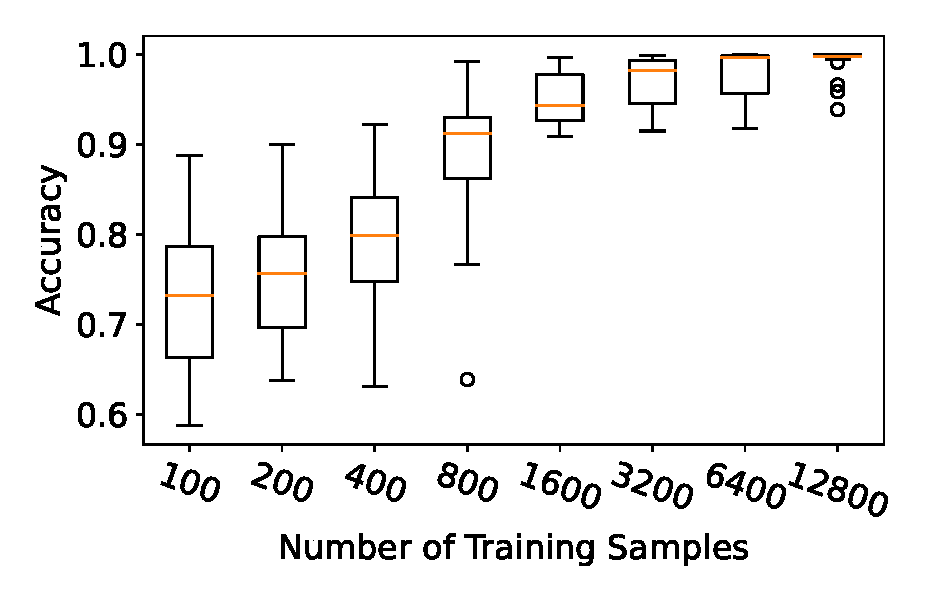
\includegraphics[width=\figwidth]{task_1/figures/num_train_box_30_2.pdf}
  \hskip 0.5mm
  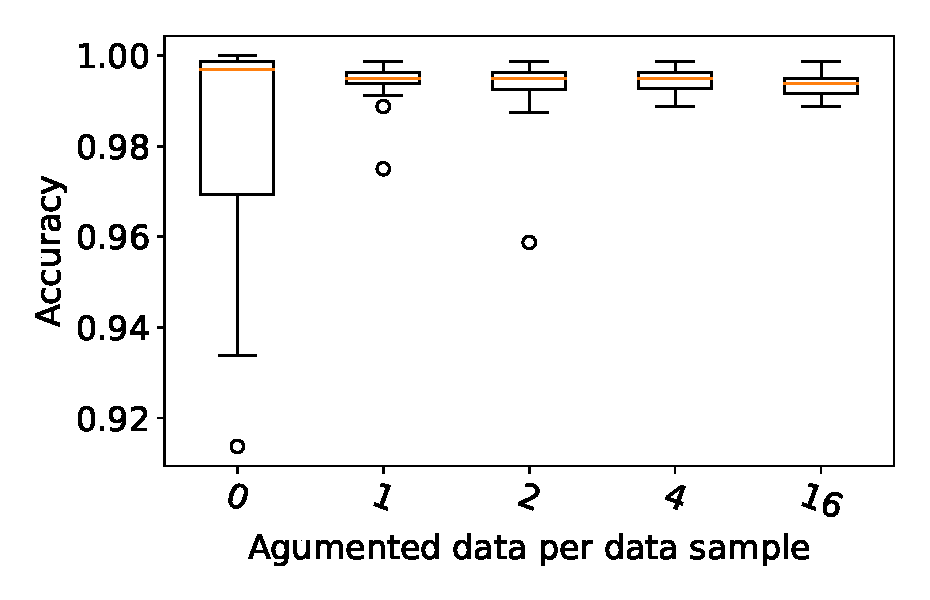
\includegraphics[width=\figwidth]{task_1/figures/ag_train_box_30_2.pdf}
  \vskip 0.5mm
  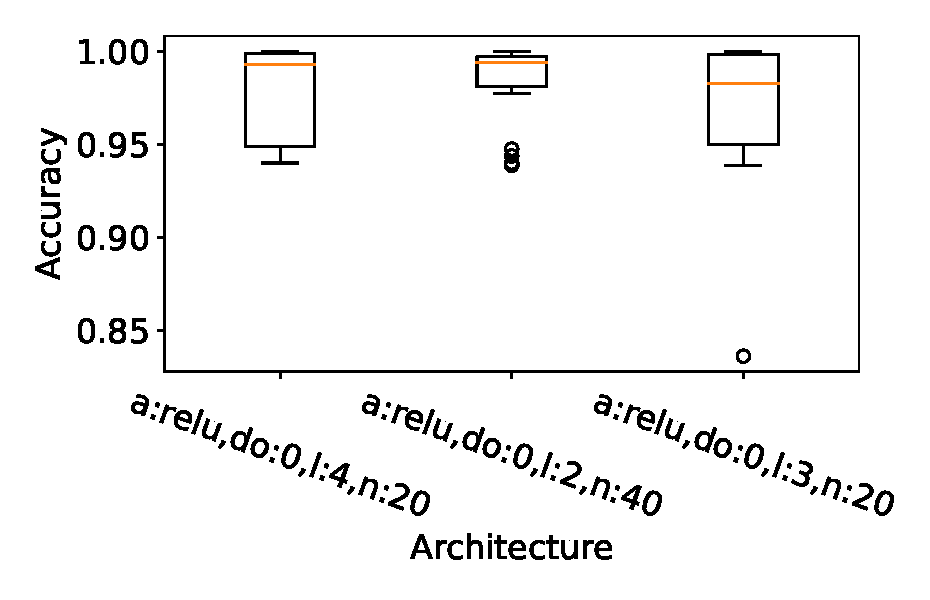
\includegraphics[width=\figwidth]{task_1/figures/architecture_box_30_2.pdf}
  \hskip 0.5mm
  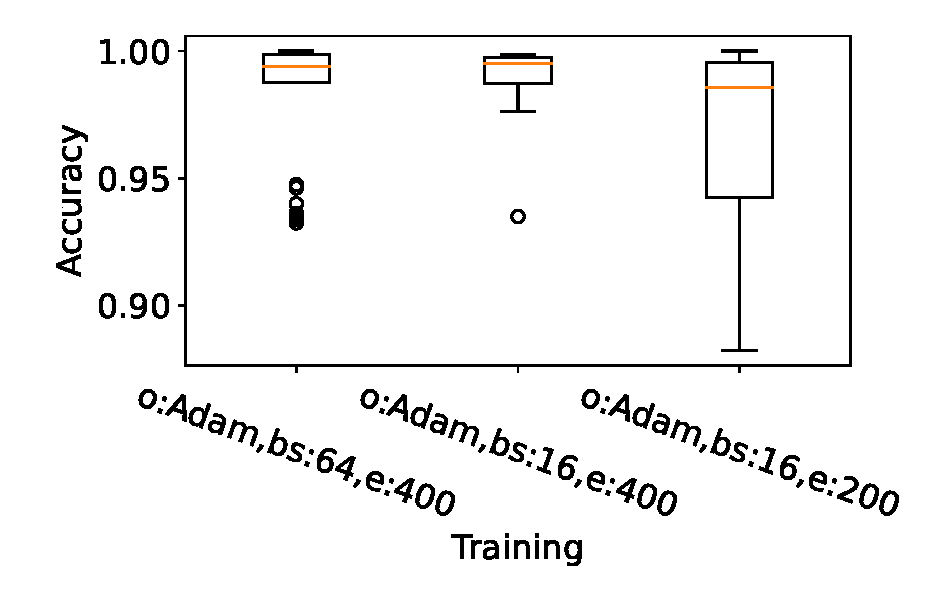
\includegraphics[width=\figwidth]{task_1/figures/training_box_30_.pdf}
  \vskip 0.5mm
  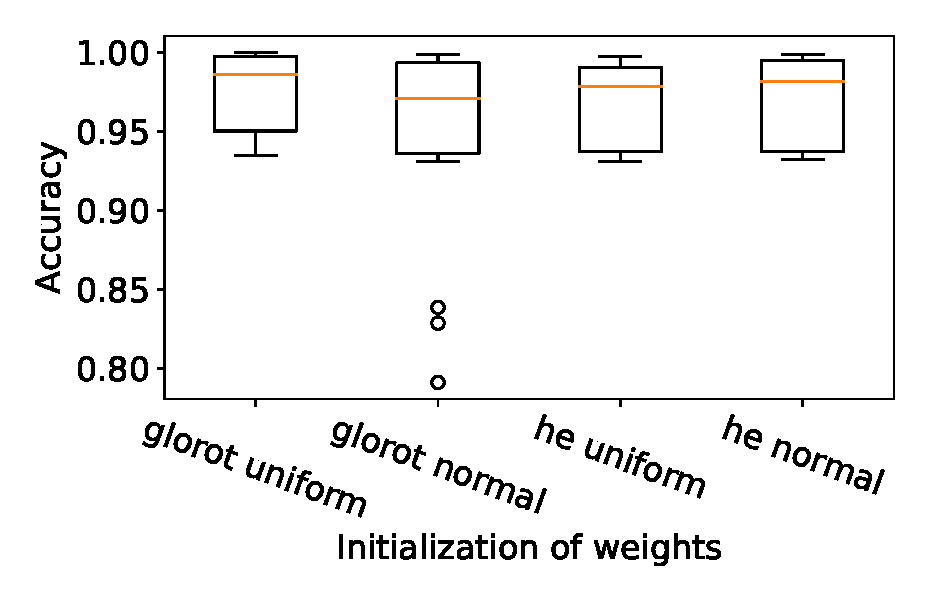
\includegraphics[width=\figwidth]{task_1/figures/init_weights_box_30_2.pdf}
  \hskip 0.5mm
  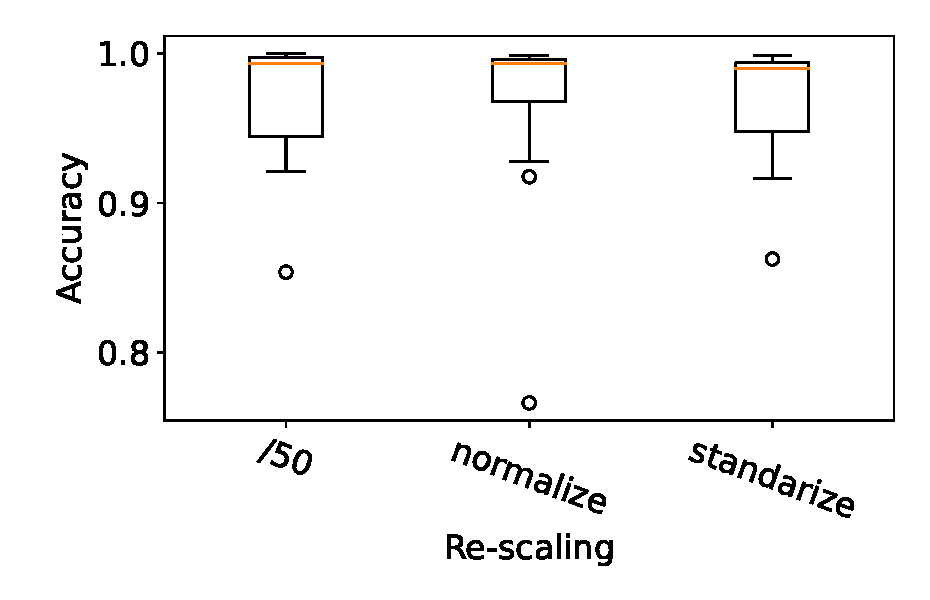
\includegraphics[width=\figwidth]{task_1/figures/rescale_box_30_2.pdf}
  \caption{The figure shows the 30 run distribution accuracies for different cases:
  (a) Different number of training samples with default network and training parameters. (b) Additional augmented samples per original training samples. (c) The three best scoring architectures found through grid search with default training parameters. The short hands are, \textbf{a} the activation of the hidden layers, \textbf{do} the dropout of each hidden layer, \textbf{l} the number of hidden layers and \textbf{n} the number of nodes in each hidden layer. (d) The three best scoring training parameters found through grid search with default architecture. The \textbf{o} is the optimizer algorithm used, \textbf{bs} is the batch size and \textbf{e} is the number of epochs used. (e) Different weight initialization distributions. (f) Different re-scaling methods.}
  \label{fig:all}
\end{figure*}


\begin{figure}[!tb]
  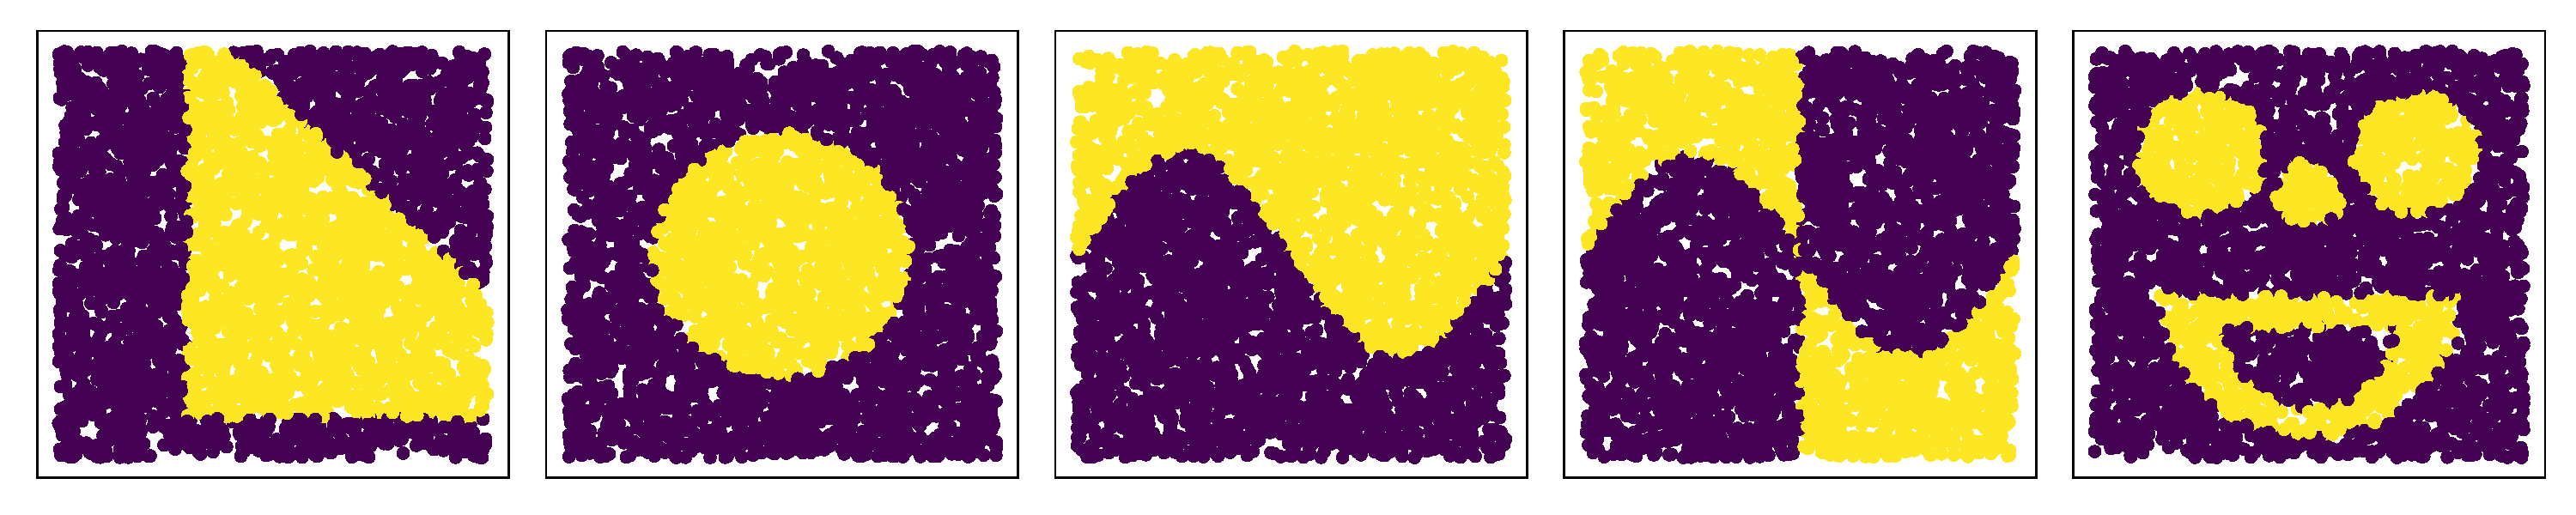
\includegraphics[width = \figwidth]{task_1/figures/non_linear_functions_2.pdf}
  \vskip 0.5mm
  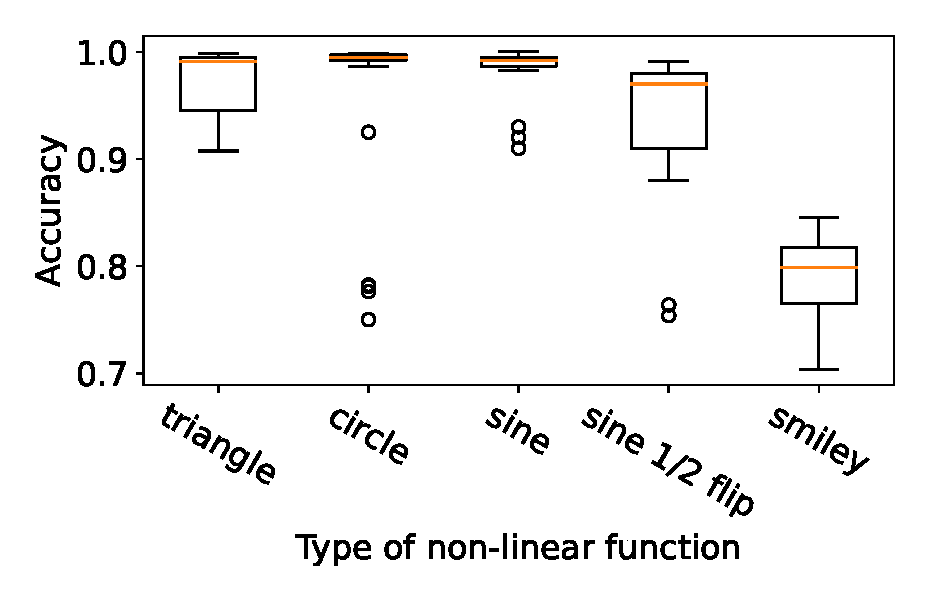
\includegraphics[width=\figwidth]{task_1/figures/types_box_30_2.pdf}
  \caption{The top row shown the non-linear functions. The lower shows the 30 run accuracy distributions for the different types of non-linear functions with the default network.}
  \label{fig:non-linear_functions}
\end{figure}
% Number of training sampels
The distribution of accuracies as a function of the number of training samples is shown in figure \ref{fig:all}(a). There was a clear correlation between number of training samples and the average accuracy, with a larger number of samples giving an increasing average accuracy. As one would expect. There was also a smaller variation in the obtained accuracies as the number of training samples increased. From the results one can conclude that $3200$ training samples is a satisfactory sample size because the larger values of training samples had a similar average and variation, even though they performed a bit better.

%Augmented data
The effect on the accuracy distributions by adding augmented data in addition to the original training data, set to $3200$ samples, is shown in figure \ref{fig:all}(b). Here one observed that the addition of extra augmented samples slightly dropped the average accuracy but greatly reduced the variation, especially when there was $4$ and $16$ augmented samples per original sample. The interesting part was to compare this with the case of training with $12800$ actual samples. One observed that the augmented data gave a similar accuracy and a smaller spread. This shows that one can improve a NN performance by adding augmented data. But given that the procedure for augmenting the data was chosen to best fit the actual problem, this was regarded as a best case scenario. 

% Grid Search Over architecture
The grid search over the architectural choices showed that several combinations yielded good results and that there were some inconsistencies in which combinations ended up being the best ones. A general trend was that the relu and elu outperformed the sigmoid as activation function in the hidden layers. Several combinations of layers and nodes provided equivalently good results. The dropout rate also had a relatively small effect compared to the activation function. There seemed to be a tendency to be better performance with the rate set to zero. This might be due to the small number of nodes in the architectures considered. The architecture and accuracy distributions of some of the best performing architectures are shown in figure \ref{fig:all}(c)

% Grid search over architectures
When searching over the training parameters the Adam and RMSprop methods achieved similar accuracies, but the Adam methods ran slightly faster. The Adagrad and vanilla gradient decent performed considerably worse than Adam and RMSprop. The number of epochs used does in general improve the accuracy as long as one does not start to overfit the data, which can be avoided by using an early stop method. The NN also seemed to have a tendency to not overfit as several had similar accuracies for training and validation samples for hundreds of epochs. The batch size was found to give best results in the range from $16$ to $64$. Having larger or smaller batch sizes lead to reduced performance. The accuracy distributions of some of the best set of training parameters are shown in figure \ref{fig:all}(d). Here it was evident that the larger amount of epochs gave smaller variation. 

% Initialization of weights
The effect of different initialization methods for the weights on the accuracies are shown in figure \ref{fig:all}(e). Here there was no real difference between the glorot uniform, he uniform and he normal. The glorot normal however performed considerably worse than the others on some occasions.

% Re-scaling
Accuracy distributions for the different re-scaling methods are presented in figure \ref{fig:all}(f). The difference between dividing by 50 and normalizing was very small as one would imagine given that they amount to roughly the same re-scaling. Standardizing also had similar performance to the two other methods and one could say that the chosen re-scaling method had little effect. 

% Different non-linear functions

When the NN was tested on different non-linear functions the achieved accuracy distributions are reported in figure \ref{fig:non-linear_functions} along with a illustration of the non-linear functions. It was evident that the more complex the function was there worse the average accuracy was. Also the variation increased with increased complexity. The performance on the smiley was considerably lower than the others and this was is most likely due to the several smaller features that are harder to train than large straight boundaries. 



\section{Conclusions}

When training a NN the number of training samples greatly effects the performance, especially in the case of limited data. A greater number of samples also increase the consistency, giving less variation in the achieved accuracy. The same effect was found from adding samples that contained small augmentations from the original samples. However, it was at the expense of a slightly lower average accuracy for the . The choice of optimizer seemed to favor either Adam or RMSprop, so the adaptive methods. The rectified linear activation functions of elu and relu, outperformed the sigmoid function. Within the reasonable choice of layers and nodes investigated most seemed to perform on a similar level. The same also holds for the dropout rate within the lower values. Most of this large amount of possible combinations is probably due to the simple nature of the problem. The performance was evidently worse on the more complex functions.







\begin{thebibliography}{99}

\bibitem{pap1}
  B. Franklin,
  J. Here There {\bf 10}, 20--40 (1800).
  
\bibitem{pap2}
  A. Einstein,
  Int. J. There Here {\bf 20}, 125--133 (1910).
  
\end{thebibliography}

\clearpage

% %%%%%%%%%%%%%%%%%%%
% \begin{figure*}[!tb]
%   \centering
%   \includegraphics[width=\textwidth]{description_assignment_LCPB_20-21.pdf}
% \end{figure*}
% %%%%%%%%%%%%%%%%%%%


\end{document}


















































\begin{figure}[ht]
  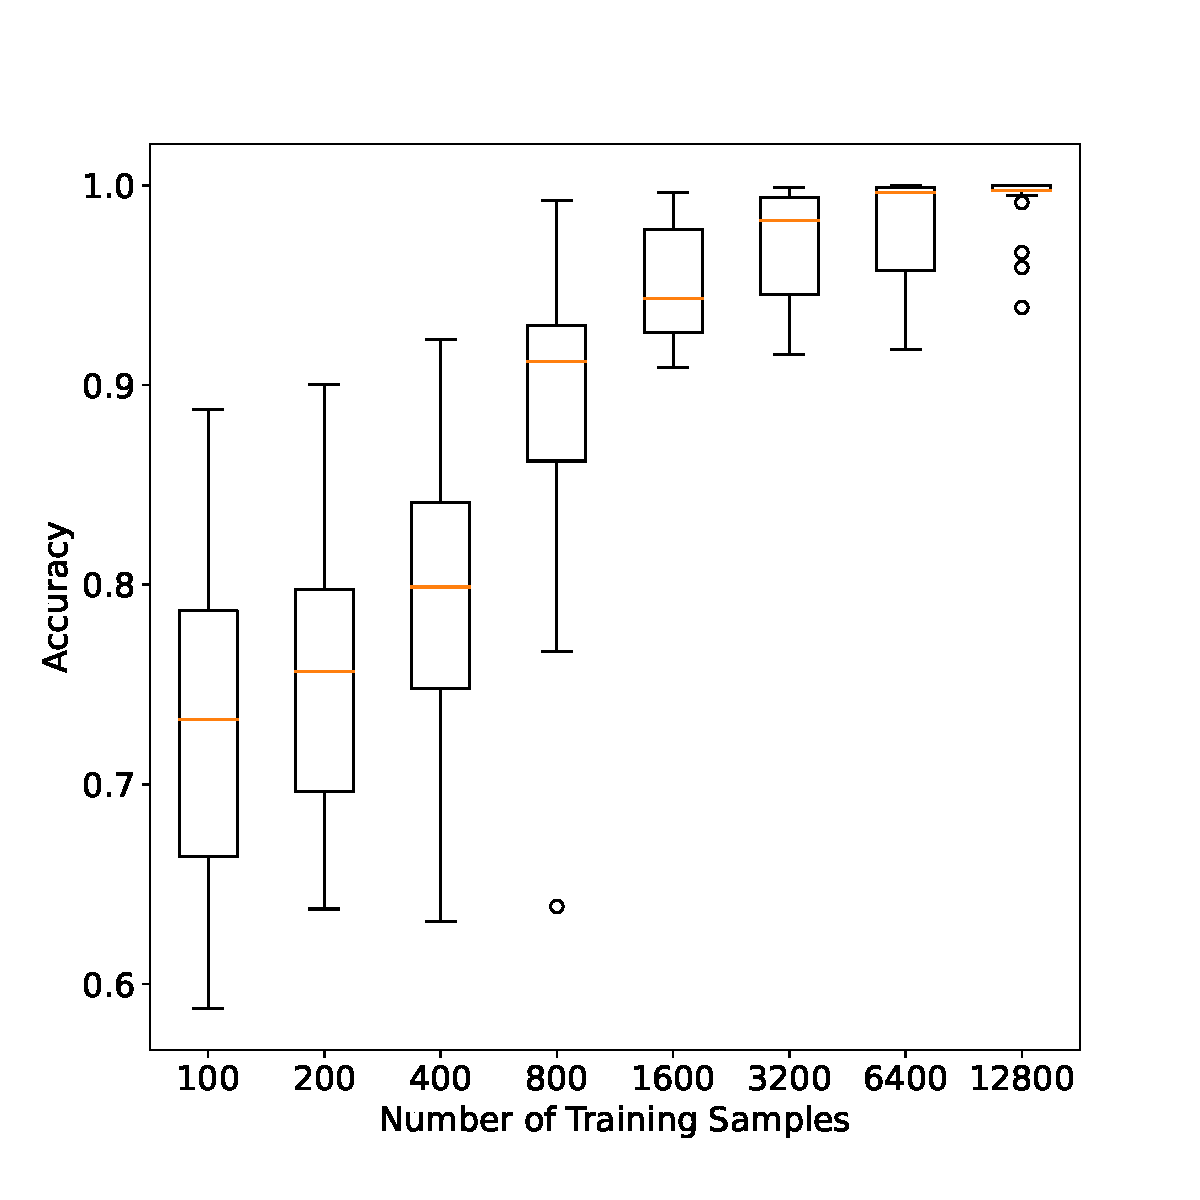
\includegraphics[width=0.44\textwidth]{task_1/figures/num_train_box_30.pdf}
  \caption{The accuracy's achieved by the default network with a varying number of training samples. Each started from 10 different initial weights.}
  \label{fig:num_train_samples}
\end{figure}


\begin{figure}[!tb]
  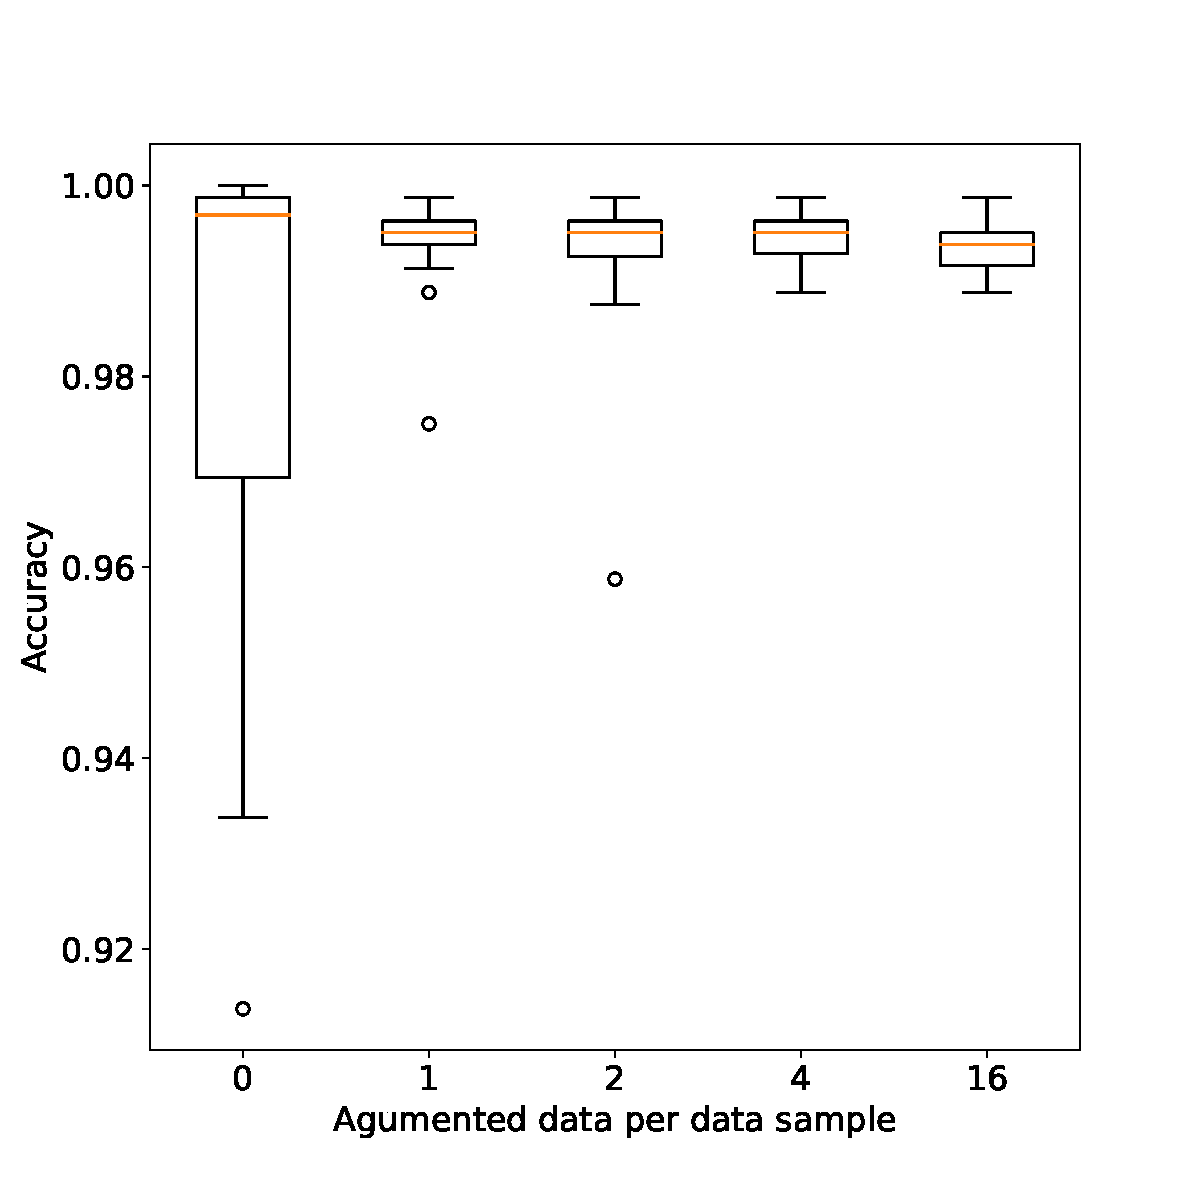
\includegraphics[width=0.44\textwidth]{task_1/figures/ag_train_box_30.pdf}
  \caption{The different accuracies achieved by the default network when adding the indicated number of augmented data per original training data. The values are for 10 different initial weights for each augmented data per original training data. The original training data consist of $3200$ samples.}
  \label{fig:augmented_train_sampels}
\end{figure}


\begin{figure}[!tb]
  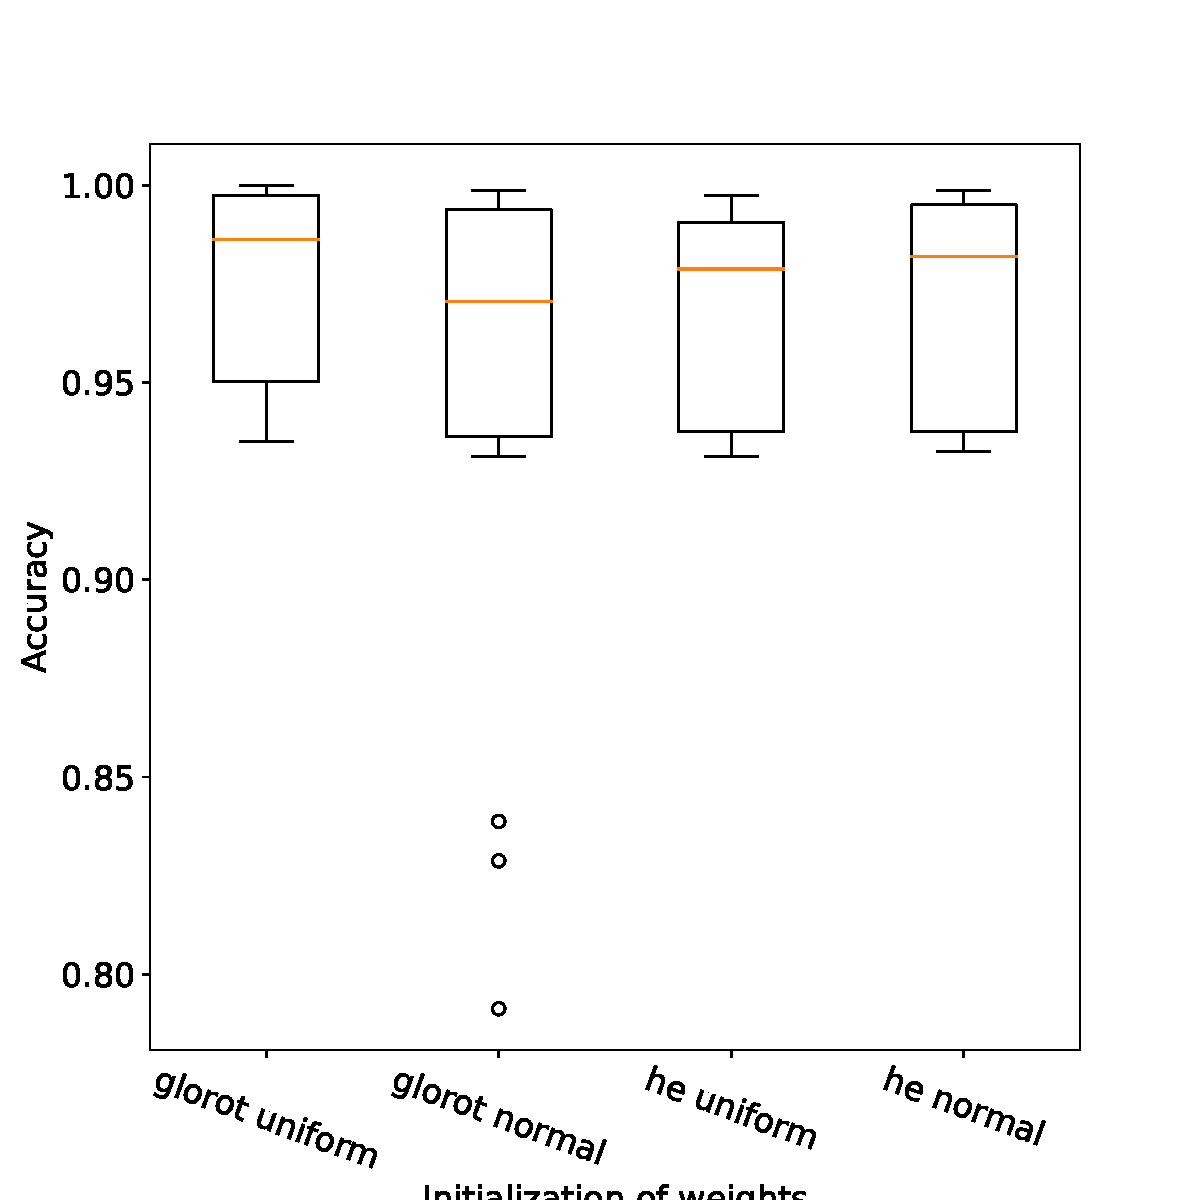
\includegraphics[width=0.44\textwidth]{task_1/figures/init_weights_box_30.pdf}
  \caption{
  The distribution of accuracies achieved with different initialization distributions. 
  }
  \label{fig:weight_init_box}
\end{figure}


\begin{figure}[!tb]
  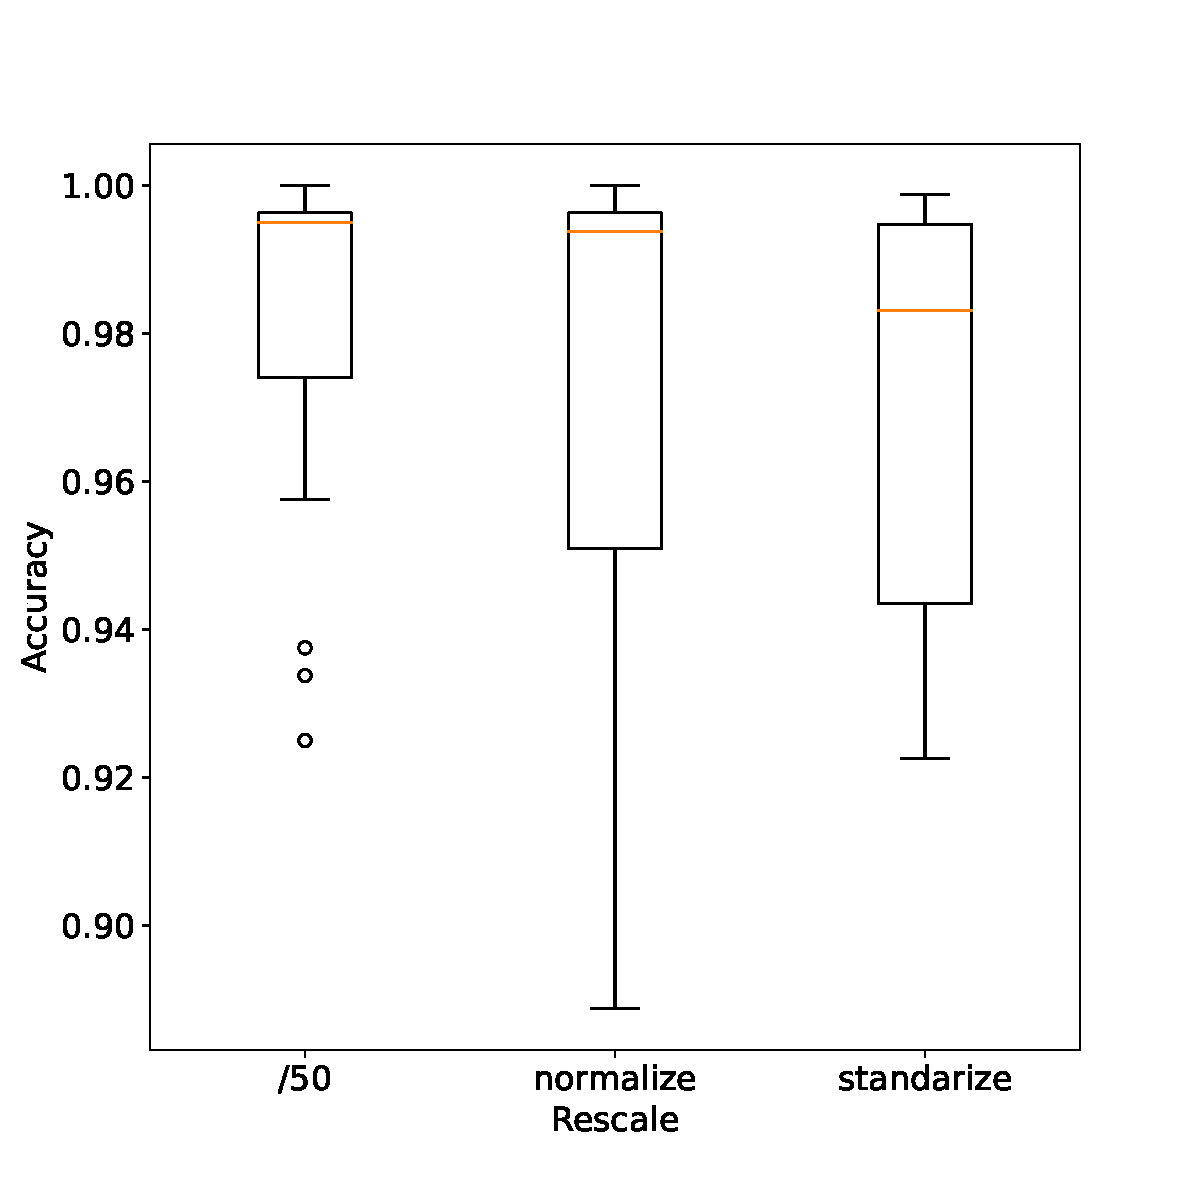
\includegraphics[width=0.44\textwidth]{task_1/figures/rescale_box_30.pdf}
  \caption{
  The distribution of accuracies achieved with different re-scaling methods. 
  }
  \label{fig:rescale_box}
\end{figure}

\begin{figure}[!tb]
  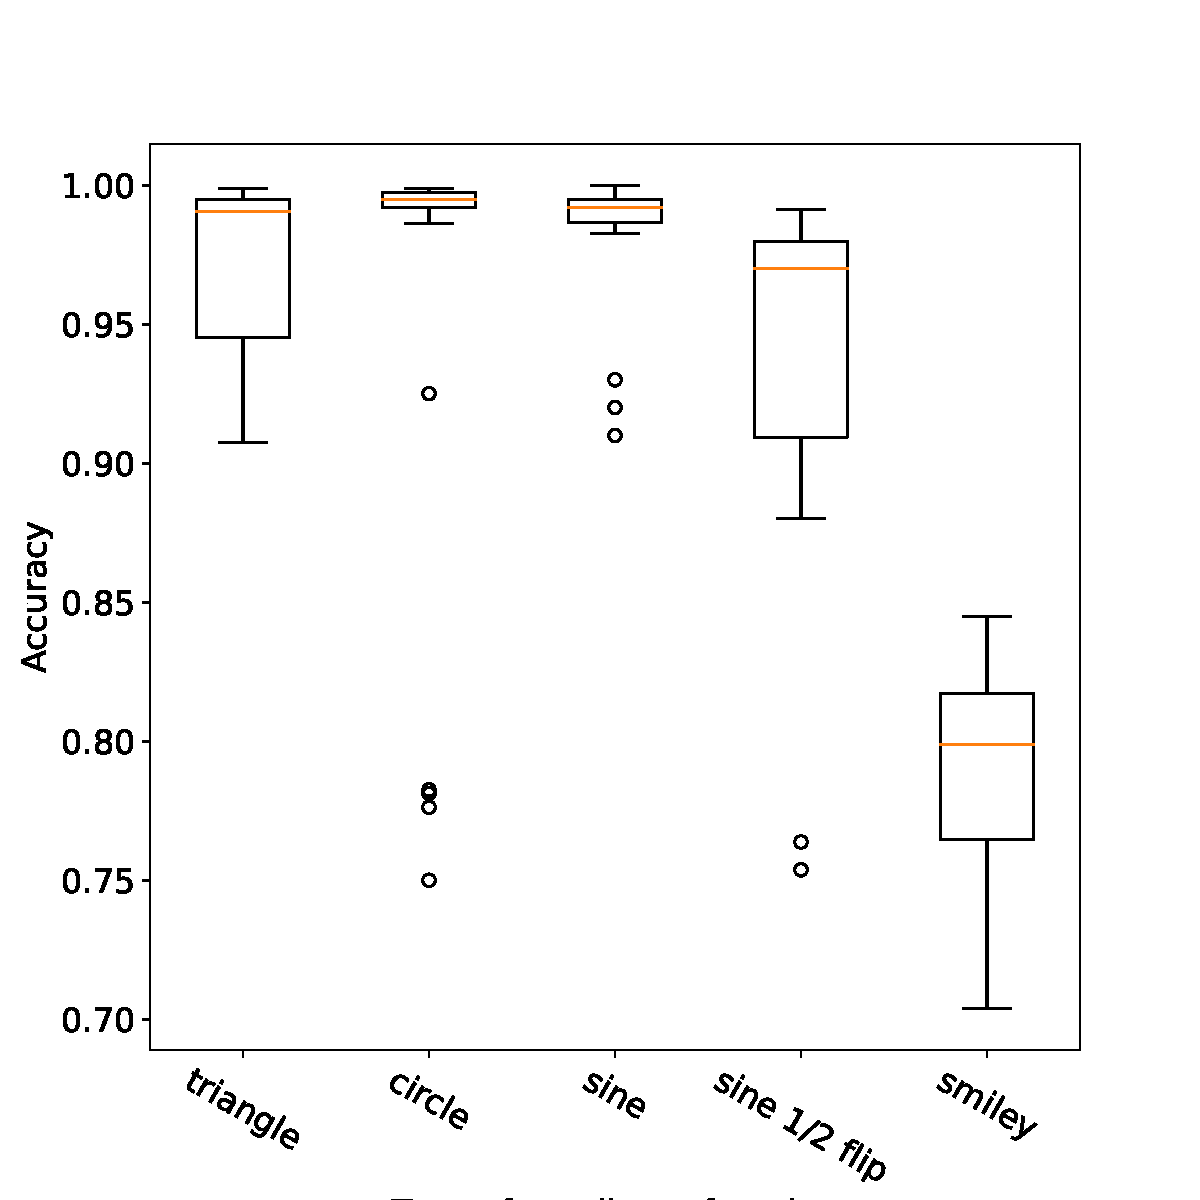
\includegraphics[width=0.44\textwidth]{task_1/figures/types_box_30.pdf}
  \caption{
  The distribution of accuracies for the different non-linear functions used to label the points. 
  }
  \label{fig:rescale_box}
\end{figure}

\begin{figure}[!tb]
  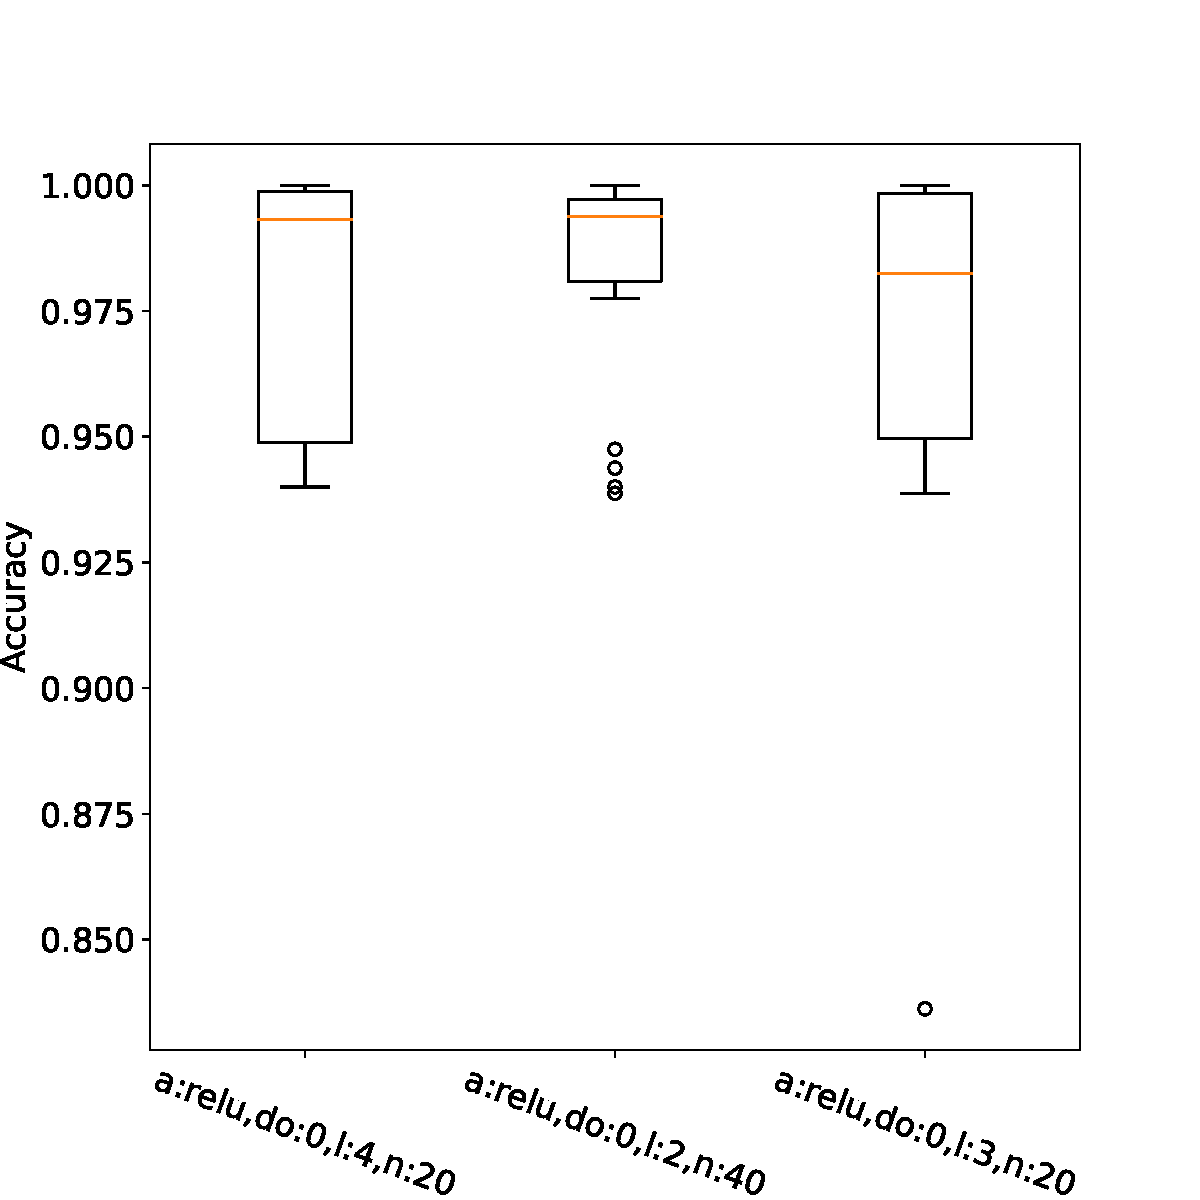
\includegraphics[width=0.44\textwidth]{task_1/figures/architecture_box_30.pdf}
  \caption{
  The three best architectures from grid search. The short hands are, a the activation of the hidden layers, do the dropout of each hidden layer, l the number of hidden layers and n the number of nodes in each hidden layer. 
  }
  \label{fig:architecture_gs_box}
\end{figure}

\begin{figure}[!tb]
  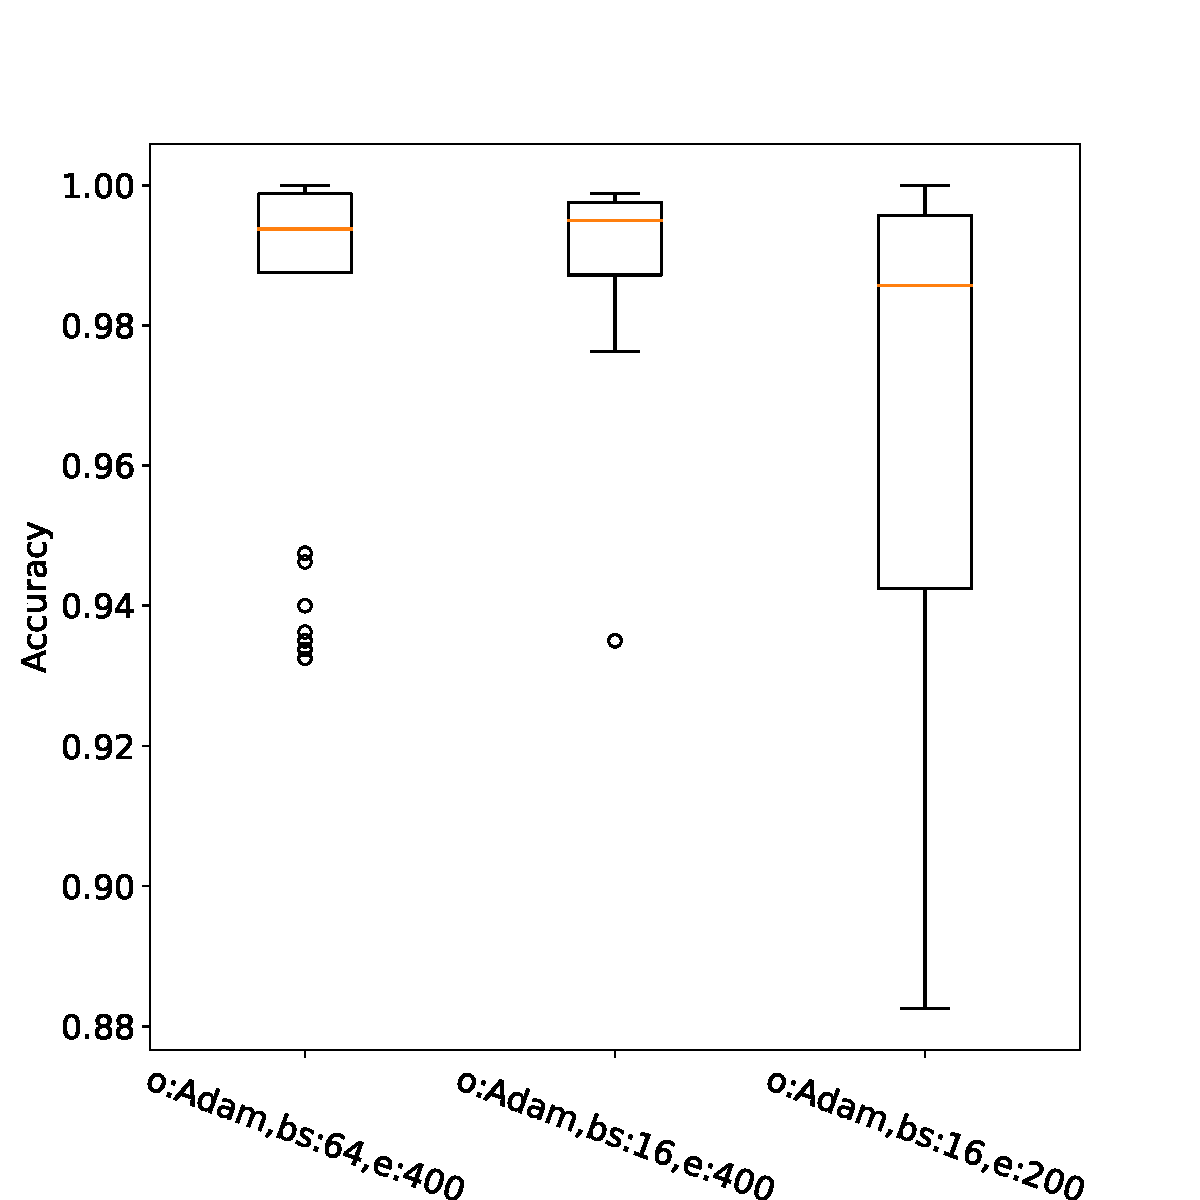
\includegraphics[width=0.44\textwidth]{task_1/figures/training_box_30.pdf}
  \caption{
  The three best training options from grid search. The o is the optimizer algorithm used, bs is the batch size and e is the number of epochs used. 
  }
  \label{fig:architecture_gs_box}
\end{figure}


\begin{figure}[!tb]
  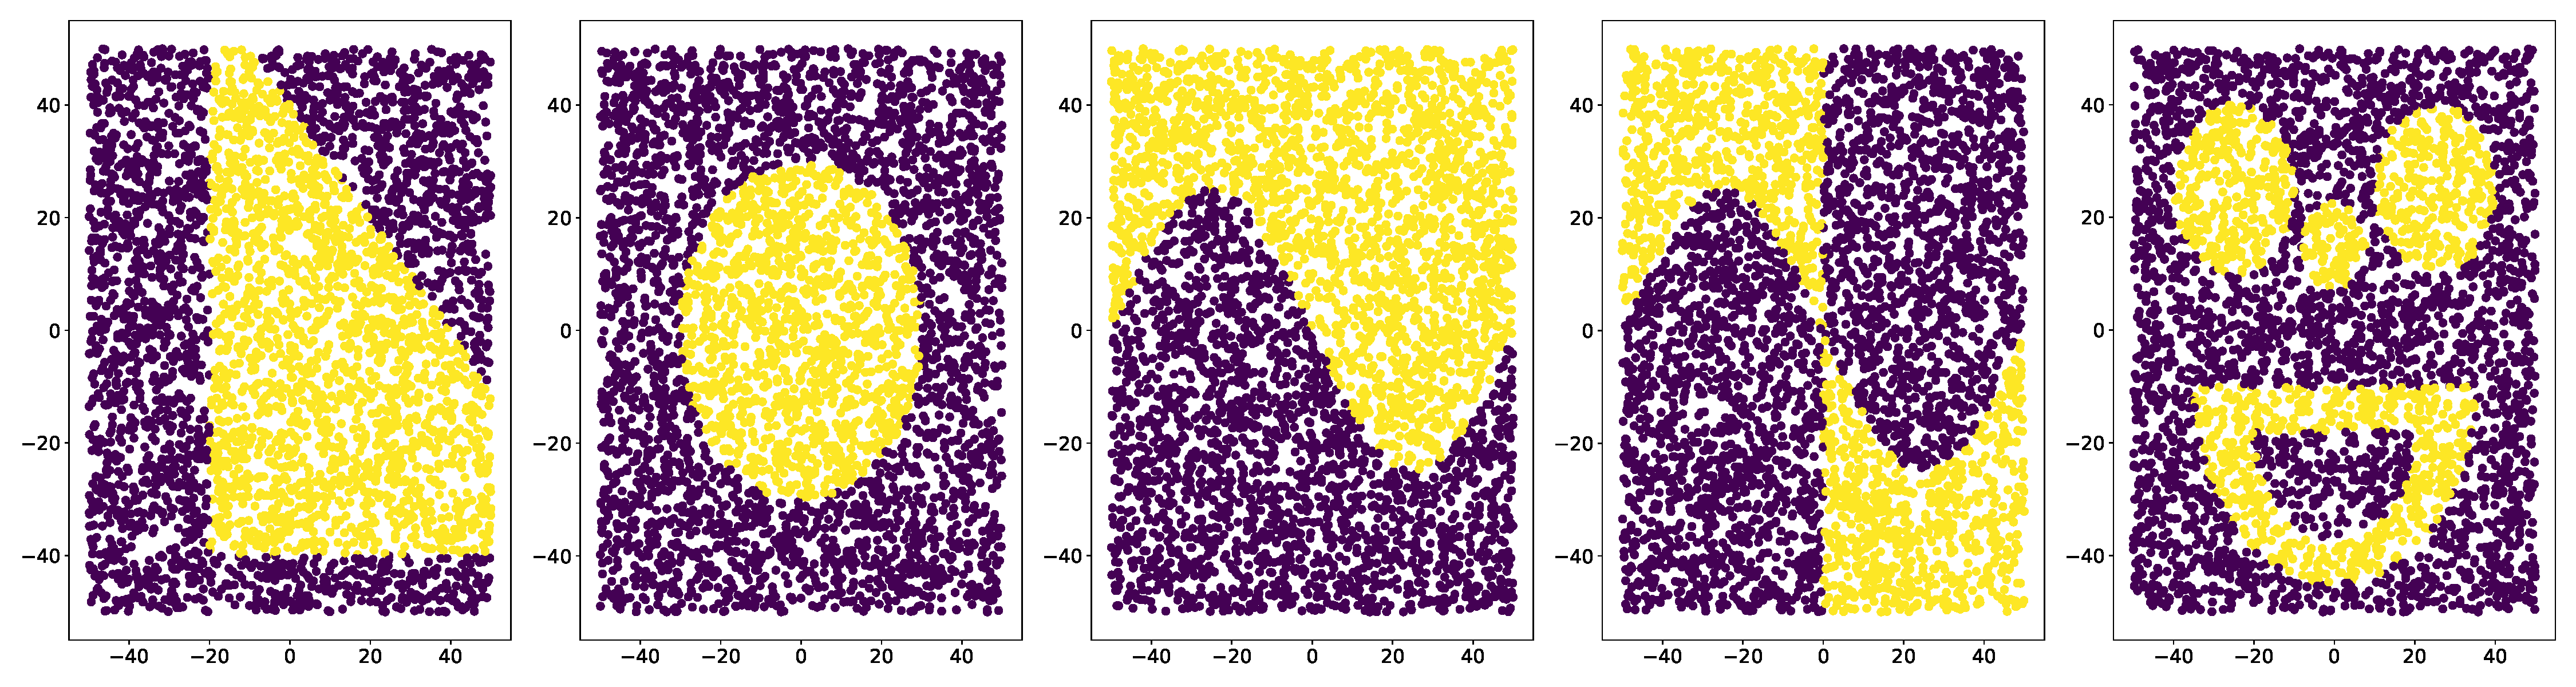
\includegraphics[width=0.50\textwidth]{task_1/figures/non_linear_functions.pdf}
  \caption{
  The five different non-linear labeling functions used. From left to right named triangle, circle, sine, sine 1/2 flip and smiley. \color{red} maby not keep \color{black}
  }
  \label{fig:rescale_box}
\end{figure}



% Templates that might be needed


\begin{table}[!b]
\begin{center}
\begin{tabular}{lll}
quantity & symbol & dimensionless \\
\hline
time & $t$ & $t'$  \\
momentum & $p$ & $v$
\end{tabular}
\end{center}
\caption{Description of the table.}
\label{tab:1}
\end{table}


\begin{table}[!b]
\begin{center}
\begin{tabular}{llllll}
\hline
accuracy(std) & time[s] & layers & nodes & dropout & afunc \\
\hline
0.977 (0.029) & 9.77 & 3 & 40 & 0.0 & relu\\
0.980 (0.026) & 9.84 & 4 & 10 & 0.0 & relu\\
0.988 (0.020) & 10.74 & 4 & 40 & 0.0& relu\\
\hline
\end{tabular}
\end{center}
\caption{The best architectures found from grid search with cross validation with 5 folds. Time is the average time used to train the network. Layers is the number of hidden layers, searched over the values 2,3,4. Nodes are the number of nodes in each hidden layer, the values used for the grid were 10,20,40. Dropout is the dropout rate of the nodes in the hidden layers. The values 0 and 0.1 were checked. Afunc is the activation function used in the hidden layers, where sigmoid, relu and elu were the alternatives. The presented accuracy is the average value when the model is trained from 10 different initial weights.}
\label{tab:grid_search_architecture}
\end{table}


\begin{table}[!b]
\begin{center}
\begin{tabular}{lllll}
\hline
accuracy(std) & batch size & epochs & optimizer \\
\hline
0.964 (0.034) & 16 & 400 & Adam\\
0.950 (0.030) & 4 & 400 & RMSpropu\\
0.961 (0.029) & 4 & 40 & 0.0& relu\\
\hline
\end{tabular}
\end{center}
\caption{The best training parameters found from grid search with cross validation with 5 folds. The presented accuracy is the average value when the model is trained from 10 different initial weights. The batch size is the number of samples used for each update. The epochs are the number of times the training set has been looped through. The optimizer is the optimizing algorithm used to train the network. The default architecture is used.}
\label{tab:grid_search_training}
\end{table}


% \subsection{Classification}
The rectangle for labeling the samples was given by the limits
\begin{equation}
f(x_1,x_2) = \begin{cases} 1,\
x_1\in [-20,80] \wedge x_2 \in [-40,80-x_1]\\
0, \ \textrm{else}
\end{cases}
\end{equation}





